%
%  Semesterarbeit Dokumentation
%
%  Created by Silvan Spross on 2010-10-21.
%
\documentclass[abstracton,liststotoc,bibtotoc]{scrreprt}
\usepackage[ngerman]{babel}

% Use utf-8 encoding for foreign characters
\usepackage[utf8]{inputenc}

% Setup for fullpage use
\usepackage{fullpage}

% Running Headers and footers
%\usepackage{fancyhdr}
 
% Multipart figures
%\usepackage{subfigure}

% More symbols
%\usepackage{amsmath}
%\usepackage{amssymb}
%\usepackage{latexsym}

% Surround parts of graphics with box
\usepackage{boxedminipage}

% Package for including code in the document
\usepackage{listings}

% If you want to generate a toc for each chapter (use with book)
\usepackage{minitoc}

% This is now the recommended way for checking for PDFLaTeX:
\usepackage{ifpdf}

\ifpdf
    \usepackage[pdftex]{graphicx}
\else
    \usepackage{graphicx}
\fi

% Package for including hyperlinks in the document
\usepackage[colorlinks=true, pdfstartview=FitV, linkcolor=black, citecolor=black, urlcolor=black]{hyperref}

\usepackage{booktabs}

\title{Webapplikation für eine öffentliche Medienbibliothek mit einer API}

\author{Studierender - Silvan Spross\\
    Projektbetreuer - Beat Seeliger\\
    \\
    HSZ-T - Technische Hochschule Zürich}
    
\date{Oktober 2010 bis Januar 2011}

\begin{document}

    \ifpdf
        \DeclareGraphicsExtensions{.pdf, .jpg, .tif}
    \else
        \DeclareGraphicsExtensions{.eps, .jpg}
    \fi
    
    \pagenumbering{Alph}

    \maketitle
    
    \begin{abstract}
    
    Test
    
\end{abstract}
    
    \pagenumbering{Roman}

    \tableofcontents
    
    \clearpage
    \pagenumbering{arabic}

    \chapter{Einleitung}
    \section{Ausgangslage}
Viele Personen sind im Besitz von digitalen Medien wie zum Beispiel Filme.
Im Internet gibt es diverse Plattformen, um detaillierte Informationen zu 
Filmen zu finden und sie zu bewerten. 

Die Inhalte werden jedoch von den Plattformbetreibern gepflegt und die 
Benutzer haben keine Möglichkeit sich wie bei Wikipedia einzubringen. Auch 
basieren die Bewertungen oft auf dem Durchschnitt aller Benutzer. Dies
führt relativ schnell zu einer unnützlichen Bewertung, da die Geschmäcker
sehr verschieden sind.

\section{Ziel der Arbeit}
Wikipedia hat bewiesen, dass öffentliches Pflegen von Inhalten 
funktioniert. In dieser Arbeit soll ein Prototyp einer Plattform erstellt
werden, wo Inhalte zu Medien frei erfasst und bearbeitet werden können.
Als weitere Neuerung sollen Benutzer die Bewertungsanzeige von Medien auf
frei definierbare Gruppen, wie zum Beispiel ihre Freunde, festlegen 
können, um so Bewertungen mit gleichem Geschmack zu sehen.

Zusätzlich soll auch der Quellcode der Plattform öffentlich verfügbar sein, 
damit auch dieser von Dritten weiter gepflegt werden kann. Dazu muss die 
Wahl der Technologien und Tools wohl überlegt sein, damit sich weitere 
Entwickler finden lassen.

\section{Abgrenzung}
Die Analysen beschränken sich auf Recherchen im Internet, Büchern und das 
nähere Umfeld des Studierenden. Es werden keine Umfragen, Erhebungen und 
Feldstudien durchgeführt. Der Prototyp wird nur über einen Bruchteil der 
Funktionalität der eigentlichen Plattform verfügen, da es den Rahmen
dieser Arbeit sprengen würde.

Die Medien wurden auf das Medium Filme beschränkt, damit für eine 
Kategorie möglichst genaue Aussagen getroffen werden können.

\section{Richtlinien}
Folgende Dokumente mit Richtlinien der Hochschule für Technik Zürich 
wurden für die Semesterarbeit berücksichtigt:

\begin{itemize}
    \item Reglement \cite{hsz_reglement}
    \item Ablauf \cite{hsz_ablauf}
    \item Bewertungskriterien \cite{hsz_bewertungskriterien}
\end{itemize}

\section{Sprache}
Die Semesterarbeit wurde in deutscher Sprache verfasst. Englische Ausdrücke 
wurden immer dort verwendet, wo diese im Sprachgebrauch in den verwendeten 
Programmen genau so gebraucht werden.

Aus Gründen der besseren Lesbarkeit der Semesterarbeit wurde teilweise auf 
die Nennung beider Geschlechter verzichtet. In diesen Fällen ist die 
weibliche Form ausdrücklich inbegriffen.

\section{Angewandte Methoden}
Folgende Methoden wurden in dieser Arbeit zur Unterstützung verwendet. 

\subsection{Nutzwertanalyse}
Die Nutzwertanalyse gehört zu den quantitativen nicht-monetären Analysemethoden 
der Entscheidungstheorie. In Form einer oder mehreren 
Entscheidungsmatrizen werden Kriterien und Argumente, welche letztendlich eine 
Entscheidung bestimmen, einer genauen Prüfung unterzogen und auf eine Auswahl 
angewandt \cite{nutzwertanalyse}.

\subsection{Wireframing}
Alternativ zum Ausdruck ``Mock-up'' wird der Begriff ``Wireframe'' benutzt, um einen 
sehr frühen konzeptuellen Prototypen einer Website oder eines Software-Frontends 
darzustellen. Bezogen auf eine Website sollten Elemente wie Navigation und 
Inhaltsbereiche Teil dieses Skeletts sein \cite{wireframe}.

\subsection{Entity Relationship Model}
Das ERM (``Entity-Relationship-Modell'') dient dazu, im Rahmen der semantischen 
Datenmodellierung einen Ausschnitt der realen Welt zu beschreiben. 
Das ER-Modell besteht jeweils aus einer Grafik und einer Erläuterung \cite{erm}.
    
    \chapter{Ist Analyse}
    \section{Konkurrenz}
Es existieren diverse Plattformen die Informationen zu Filmen zur Verfügung stellen.
Die laut Google \cite{movie_informations} Bekannteste unter ihnen ist ``The Internet Movie Database'',
besser bekannt unter der Abkürzung ``IMDB''. Sie bietet detaillierte Informationen
zu existierenden Filmen, solche die zur Zeit gedreht werden und sogar über jene, die
sich erst in der Planungsphase befinden.

Es existieren natürlich noch viele weitere Plattformen und die Grössten unter 
ihnen möchte ich nach den folgenden drei Kriterien beurteilen:

\begin{table}[h]
\begin{center}
    \begin{tabular}{lp{12cm}l}
        \toprule Nr & Beschreibung \\
        \midrule 1 & Der Besucher kann die Beschreibung, welche den Inhalt 
                     des Films in einer kurzen Zusammenfassung wiedergibt, mitbestimmen. \\
        \midrule 2 & Der Besucher kann die Filme bewerten. \\
        \midrule 3 & Der Besucher hat die Möglichkeit für jeden Film eine zusätzliche
                     Bewertung zu sehen, die nur über ihn und seine Freunde berechnet
                     wird und somit für seinen Geschmack aussagekräftiger ist. \\
        \bottomrule
    \end{tabular}
    \caption{Bewertungskriterien einer guten Filmbewertungsplattform}
    \label{tab:bewertungskriterien}
\end{center}
\end{table}

Der Prototyp namens ``OpenMediaLibrary'', kurz ``OML'', der in dieser Arbeit erstellt werden soll, 
soll alle drei Kriterien erfüllen, da diese meines Erachtens die Grundlage für eine gute 
öffentliche Filmdatenbank sind.

In der Tabelle \ref{tab:plattformen} habe ich die bekannteren und unbekannteren 
Plattformen untersucht und nach den definierten Kriterien beurteilt. Ein `x' bedeutet,
dass die Plattform das Kriterium erfüllt und ein `-', dass sie es nicht erfüllt.

\begin{table}[h]
\begin{center}
    \begin{tabular}{lllccc}
        \toprule Nr & Name & URL & \multicolumn{3}{c}{Kriterien} \\ & & & 1 & 2 & 3 \\
        \midrule 1 & The Internet Movie Database & imdb.com & - & x & - \\
        \midrule 2 & Deutsche Film- und Medienbewertung & fbw-filmbewertung.com & - & - & - \\
        \midrule 3 & Online-Filmdatebank & ofdb.de & - & x & - \\
        \midrule 4 & Wikipedia & wikipedia.com & x & - & - \\
        \midrule 5 & Rotten Tomatoes & rottentomatoes.com & - & x & - \\
        \bottomrule
    \end{tabular}
    \caption{Existierende Plattformen}
    \label{tab:plattformen}
\end{center}
\end{table}

Wie in der Ausgangslage schon angenommen hat die Recherche ergeben, dass nur
wenige Plattformen die Mitarbeit der Besucher erlaubt. Fast alle bieten
eine Bewertung an, jedoch keine eine Bewertung die sich nur auf den
Freundeskreis des Betrachters bezieht.

\section{Funktionsumfang}
Relevant sind jedoch nicht nur meine Bewertungskriterien aus der Tabelle \ref{tab:bewertungskriterien},
sondern auch der allgemeine Funktionsumfang einer Filmbewertungsplattform.
Deshalb bewerte ich die Plattformen inklusive der geplanten neuen Plattform ``OML'' 
anhand von mir ausgewählten Funktionen, die ich dann mit einer Gewichtung,
im Hinblick auf was eine gute und öffentliche Plattform auszeichnet, versehe.

Folgende sechs Funktionen sind meines Erachtens die Basis einer solchen Plattform: 

\begin{enumerate}
    \item \textbf{Filmbeschreibung}\\
          Ein Film hat eine Beschreibung, welche ohne jegliche Kritik den Inhalt
          des Filmes in einer kurzen Zusammenfassung wiedergibt. Bei dieser Funktion
          wird jedoch nicht darauf geachtet, ob der Benutzer darauf Einfluss nehmen
          kann oder nicht.
    \item \textbf{Redaktionelle Bewertung}\\
          Ein Film hat eine Bewertung, die von den Verfassern der Filmbeschreibung 
          abgegeben wird. Also keine berechnete, sondern eine subjektive Bewertung
          des oder der Autoren der Filmbeschreibung.
    \item \textbf{Bewertung durch Benutzer}\\
          Ein Film kann durch die Benutzer, die sich auf der Plattform
          registrieren müssen, bewertet werden. Die Bewertungen aller Benutzer
          fliessen dann in eine Gesamtbewertung. Die Gesamtbewertung wird berechnet,
          indem man den Mittelwert der Summe aller Bewertungen nimmt.
    \item \textbf{Kommentare von Benutzern}\\
          Benutzer können individuelle Kommentare zu einen Film abgeben. Diese
          können ergänzend zu einer Bewertung, aber auch ohne, hinzugefügt werden.
    \item \textbf{Bewertung des Freundeskreises}\\
          Ein Benutzer kann die Bewertung eines Filmes im Kreise seiner Freunde
          betrachten und so eine, für ihn, aussagekräftigere Bewertung erhalten.
          Diese wird berechnet, indem man den Mittelwert der Summe aller Bewertungen
          seiner Freunde und seiner eigenen nimmt.
    \item \textbf{Weiterführende Informationen}\\
          Es können weitere Verweise und Hinweise, die nützliche Informationen
          zu einem Film bieten, abgebildet werden. Dies kann in Form von zusätzlichen
          Quellenangaben, Kaufinformationen oder rein informativen Texten sein.
\end{enumerate}

\subsection{Gewichtung}
Nun versehe ich die genannten Funktionen mit einer Gewichtung. Diese spiegelt die
Relevanz der Funktion wieder. Die Gewichtung ist von mir vergeben, jedoch in Bezug
auf Diskussionen in meinem näheren Umfeld.

In der Tabelle \ref{tab:funktionen} habe ich die Funktionen und deren Gewichtung
aufgelistet. Die Gewichtung geht von 1 bis 5, wobei 1 für `unwichtig' und 5 für
`sehr wichtig' steht. Es dürfen nur ganze Zahlen verwendet werden, da ich 
absichtlich eine Gewichtung ohne exakte Mitte gewählt habe. Dies dient der
Aussagekraft und der besseren Abgrenzbarkeit.

\begin{table}[h]
\begin{center}
    \begin{tabular}{llc}
        \toprule Nr & Funktion & Gewichtung \\
        \midrule 1 & Filmbeschreibung & 5 \\
        \midrule 2 & Redaktionelle Bewertung & 2 \\
        \midrule 3 & Bewertung durch Benutzer & 4 \\
        \midrule 4 & Kommentare von Benutzern & 1 \\
        \midrule 5 & Bewertung des Freundeskreises & 4 \\
        \midrule 6 & Weiterführende Informationen & 3 \\
        \bottomrule
    \end{tabular}
    \caption{Funktionen einer guten Filmbewertungsplattform}
    \label{tab:funktionen}
\end{center}
\end{table}

\subsection{Direkter Vergleich}
Nun übertrage ich die Funktionen inklusive Gewichtung auf die einzelnen Plattformen
um die bestehenden mit der geplanten Plattform vergleichen zu können.

Als vergleichbare Grundlage habe ich bei den bestehenden Plattformen den Film 
``Das Experiment'' aus dem Jahre 2001 gewählt. In der Tabelle \ref{tab:deeplinks} 
sind die genauen Webadressen zu dem Film auf den einzelnen Plattformen aufgelistet. 
Die Deeplinks sind zum Zeitpunkt der Erstellung dieser Arbeit gültige Adressen.

\begin{table}[h]
\begin{center}
    \begin{tabular}{lll}
        \toprule Plattform & Deeplink \\
        \midrule 1 & \url{http://www.imdb.com/title/tt0250258/} \\
        \midrule 2 & \url{http://www.fbw-filmbewertung.com/film/das_experiment_1} \\
        \midrule 3 & \url{http://www.ofdb.de/film/3681,Das-Experiment} \\
        \midrule 4 & \url{http://de.wikipedia.org/wiki/Das_Experiment_%28Film%29} \\
        \midrule 5 & \url{http://www.rottentomatoes.com/m/1116582-experiment/} \\
        \bottomrule
    \end{tabular}
    \caption{Deeplinks zu ``Das Experiment'' der existierenden Plattformen}
    \label{tab:deeplinks}
\end{center}
\end{table}

Wenn eine Plattform die gewünschte Funktion unterstützt, erhält sie die volle Gewichtung,
wenn nicht erhält sie den Wert `0'. Somit wird der Erfüllungsgrad der einzelnen Plattformen
immer als `erfüllt' oder `nicht erfüllt' angesehen. Zur bessere Darstellung wird der Wert `0' 
mit einem `-' eingetragen.

Die Bewertung der eigenen geplanten Plattform Nr. 6 ``OpenMediaLibrary'', basiert auf
der Annahme, dass alle Funktionen umgesetzt werden können, ausser die Funktionalität Nr. 6 
``Weiterführende Informationen''. Auf diese habe ich ganz verzichtet, da sie zu Beginn 
nicht zwingend notwendig ist und damit nicht die volle Punktzahl von 19 erreicht wird.

In der nachstehenden Tabelle \ref{tab:funktionen_vergleich} sind die Plattformen und
die Funktionen in einer Matrix aufgelistet und mit den Gewichtungen versehen. Als
Resultat dient die Summe der Gewichtungen pro Plattform. Um so höher die Summe, umso
mehr relevante Funktionen sind in der Plattform abgebildet.

\begin{table}[h]
\begin{center}
    \begin{tabular}{llccccccc}
        \toprule
        \multicolumn{2}{c}{Plattform} & \multicolumn{6}{c}{Funktion} & \textbf{Summe} \\
        \multicolumn{2}{c}{} & 1 & 2 & 3 & 4 & 5 & 6 & \\ 
        \midrule 1 & The Internet Movie Database & 5 & - & 4 & 1 & - & 3 & \textbf{13} \\
        \midrule 2 & Deutsche Film- und Medienbewertung & 5 & 2 & - & - & - & - & \textbf{7} \\ 
        \midrule 3 & Online-Filmdatebank & 5 & - & 4 & - & - & 3 & \textbf{12} \\ 
        \midrule 4 & Wikipedia & 5 & 2 & - & - & - & 3 & \textbf{10} \\ 
        \midrule 5 & Rotten Tomatoes & 5 & 2 & 4 & 1 & - & - & \textbf{12} \\ 
        \midrule 6 & OpenMediaLibrary & 5 & 2 & 4 & 1 & 4 & - & \textbf{16} \\ 
        \bottomrule
    \end{tabular}
    \caption{Funktionsvergleich der Plattformen}
    \label{tab:funktionen_vergleich}
\end{center}
\end{table}

\section{Konklusion}
Aus den einzelnen Summen in der Tabelle \ref{tab:funktionen_vergleich} geht hervor,
dass es sich lohnt, den Prototypen der neuen Plattform namens ``OpenMediaLibrary'' zu erstellen. 
Ich stütze mich hierbei, wie erwähnt, vor allem auf mein näheres Umfeld, wo diese Funktionalität 
ebenso gewünscht und geschätzt wird.

Falls dieses Projekt über den Prototyp-Status weiterverfolgt werden sollte, lohnt
es sich eine breitere, wenn möglich, weltweite Umfrage über den Funktionsumfang
durchzuführen.
    
    \chapter{Konzeption}
    \section{Funktionen}
Aus der Ist-Analyse und den eigenen Vorstellungen der neuen Plattform ergibt
sich ein Funktionsumfang, der im Prototyp umgesetzt werden soll. Diese
wiederum unterteile ich in `Muss' und `Kann' Funktionen. Erstere sollen
zwingend im Prototypen umgesetzt werden, die anderen behalte ich mir vor, je
nach noch zur Verfügung stehender Zeit umzusetzen oder nicht.

\subsection{Muss-Funktionen}
In der nachstehenden Tabelle \ref{tab:muss_funktionen} sind alle umzusetzenden 
Funktionen aufgelistet, nummeriert und näher beschrieben:

\begin{table}[h]
\begin{center}
    \begin{tabular}{llp{8cm}l}
        \toprule Nr & Funktion & Beschreibung \\
        \midrule 1 & Registrierung & Ein neuer Benutzer kann sich auf der Plattform
                     mit einem Benutzernamen und Passwort registrieren. \\
        \midrule 2 & Anmeldung & Ein registrierter Benutzer kann sich auf der
                     Plattform mit seinem Benutzernamen und Passwort anmelden. \\
        \midrule 3 & Filme verfassen & Filme können von Besuchern und angemeldeten Benutzern
                     betrachtet, erfasst, editiert und gelöscht werden. \\
        \midrule 4 & Bewertung sehen & Bewertungen können von Besuchern und angemeldeten Benutzern
                     betrachtet werden. \\
        \midrule 5 & Bewertung abgeben & Benutzer können eine Bewertung zu einem Film mit oder ohne
                     Kommentar abgeben. \\
        \midrule 6 & Bewertung Freundeskreis & Angemeldete Benutzer sehen zur normalen Bewertung zusätzlich
                     die Bewertung ihres Freundeskreises. \\
        \midrule 7 & Internationalisierung & Alle Inhalte können in deutscher und englischer
                     Sprache erfasst werden \\
        \midrule 8 & Schnittstelle & Die Funktionen 3 und 4 stehen ebenfalls in einer API 
                     zur Verfügung. \\
        \bottomrule
    \end{tabular}
    \caption{Zwingend umzusetzende Funktionen des Prototypen}
    \label{tab:muss_funktionen}
\end{center}
\end{table}

Anmerkung zur Funktion Nr. 7: Eine API (Application-Programming-Interface), auf 
Deutsch ``Programmierschnittstelle'', ist ein Programmteil, der von einem Softwaresystem 
anderen Programmen zur Anbindung an das System zur Verfügung gestellt wird \cite{api}.

Der Prototyp soll es anderen Programmen über diese Schnittstelle ermöglichen,
Filme und deren Bewertung abzurufen, zu ändern und zu löschen.

\subsection{Kann-Funktionen}
In der nachstehenden Tabelle \ref{tab:kann_funktionen} sind alle optional 
umzusetzenden Funktionen aufgelistet, nummeriert und näher beschrieben.

Damit die `Muss' und `Kann' Funktionen nicht miteinander verwechselt werden 
können, wird die Nummerierung fortlaufend durchgeführt.

\begin{table}[h]
\begin{center}
    \begin{tabular}{llp{8cm}l}
        \toprule Nr & Funktion & Beschreibung \\
        \midrule 9 & Freunde verwalten & Angemeldete Benutzer können Freunde
                     zu ihrer Freundesliste hinzufügen und entfernen. \\
        \midrule 10 & Bewertungen verwalten & Angemeldete Benutzer können
                     in einer spezial Ansicht alle ihre abgegebenen Bewertungen
                     und Kommentare zu Filmen bearbeiten und löschen. \\
        \midrule 11 & Favoritenliste & Angemeldete Benutzer können Filme ihrer
                     Favoritenliste hinzufügen und entfernen. \\
        \midrule 12 & Erweiterte Schnittstelle & Alle restlichen Funktionen
                     können ebenfalls, wenn nötig mit Authentifizierung, über
                     die API verwaltet werden. \\
        \bottomrule
    \end{tabular}
    \caption{Optional umzusetzende Funktionen des Prototypen}
    \label{tab:kann_funktionen}
\end{center}
\end{table}

\section{Ansichten}
Jene Funktionen, die für den Benutzer direkt abgebildet werden müssen, habe
ich in Wireframes \cite{wireframe} abgebildet, damit die eigentliche Umsetzung 
einfacher fällt.

\subsection{Grundlayout}
Als Basis einer Webapplikation dient ein gut durchdachtes Grundlayout, welches
Funktionen und Informationen, die jederzeit zur Verfügung stehen müssen, darstellt.
Wie zum Beispiel die Navigation, eine Registrier- und Anmeldefunktion und der Sprachwechsel.

In der Grafik \ref{01_grundlayout} ist ein Browserfenster abgebildet, das die
fiktive Adresse \url{http://oml.orwell.ch/} aufgerufen und geladen hat. Auf der Grafik
ist die Navigation mit drei fiktiven Menüpunkten, zwei zur Verfügung stehenden 
Sprachen und einem Registrierungs- und Anmeldebutton zu sehen. Auch ist klar erkennbar,
wo sich der Inhalt der jeweiligen Seiten befinden wird. Zusätzlich sieht man, welches
Menü und welche Sprache zur Zeit aktiv ist.

In den folgenden Ansichten wird jeweils der Seiteninhalt näher spezifiziert. Die
aktiven und inaktiven Menüs werden ebenfalls der aktuellen Seite angepasst.

\subsection{Registrierung}
In der Grafik \ref{02_registrierung} ist die Registrierung abgebildet. Um sich
auf der Plattform zu registrieren benötigt man einen Benutzername, der gleichzeitig
die E-Mailadresse des Benutzers ist. Hinzu kommt ein Passwort, dass man zur 
Bestätigung wiederholt eingeben muss.

\subsection{Anmeldung}
Nachdem man sich erfolgreich registriert hat, kann man sich auf der Plattform
mit dem Benutzernamen und Passwort anmelden. Wie diese Anmeldung aussehen soll, sieht
man in der Grafik \ref{03_anmeldung}.

\subsection{Filme}
Für die Darstellung der Filme gibt es vier verschiedene Ansichten:

\begin{enumerate}
    \item Übersicht und Auflistung aller vorhandenen Filme
    \item Detailansicht der Filme für Gäste und nicht angemeldete Benutzer
    \item Detailansicht der Filme für angemeldete Benutzer
    \item Bearbeitungsmaske des Filmes
\end{enumerate}

\subsubsection{1. Filmübersicht}
In der Grafik \ref{04_01_uebersicht} ist die erste Ansicht abgebildet. Es werden
alle vorhandenen Filme mit Namen aufgelistet. Zu jedem Film sind drei weiterführende
Funktionen verfügbar:

\begin{itemize}
    \item Details: Führt zur Detailansicht des Filmes
    \item Bearbeiten: Führt zur Bearbeitungsmaske des Filmes
    \item Löschen: Entfernt den Film von der Plattform
\end{itemize}

Zusätzlich zur Auflistung existiert ein Button zur Erstellung eines neuen Filmes.
Ich verzichte auf die Maske zur Erstellung eines neuen Filmes, da diese genau gleich
aussehen wird wie die Bearbeitungsmaske, jedoch ohne bestehendem Inhalt.

\subsubsection{2. Filmdetailansicht}
In der Grafik \ref{04_02_detail} sieht man die Detailansicht eines Filmes inklusive Bewertung
über alle Benutzer. Diese Angaben, wie auch die Filmübersicht, sind für Gäste und
unangemeldete Benutzer sichtbar.

\subsubsection{3. Filmdetailansicht für angemeldete Benutzer}
Die zusätzlichen Funktionen wie die Maske zur Abgabe einer Bewertung und die Bewertungsangabe des Filmes 
seiner Freunde sehen nur angemeldete Benutzer und ist in der Grafik \ref{04_03_detail_angemeldet} 
ersichtlich. Die Maske um eine Bewertung abzugeben ist zudem nur zu sehen, sofern der angemeldete
Benutzer noch keine Bewertung abgegeben hat. In diesem Falle würde der Benutzer an dieser
Stelle seine eigene Bewertung sehen und könnte diese bearbeiten oder entfernen.

\subsubsection{4. Bearbeitungsmaske eines Filmes}
In dieser Ansicht kann man den Namen und die Beschreibung des Filmes bearbeiten.
Wie diese aussehen soll, sieht man in der Grafik \ref{04_04_edit}.

\begin{figure}[p]
    \begin{center}
        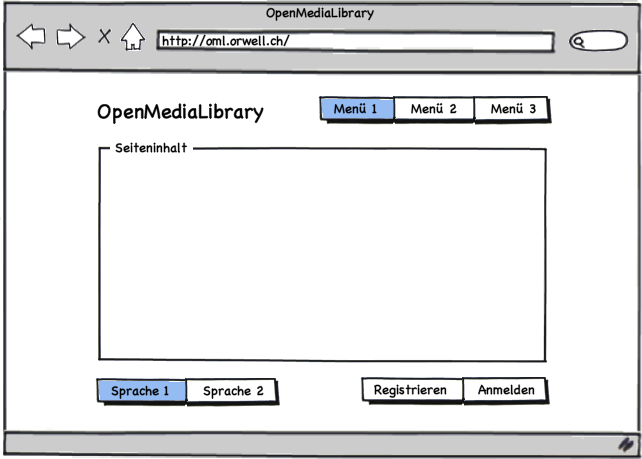
\includegraphics[width=1\textwidth,angle=0]{./wireframes/01_grundlayout.png}
        \caption{Wireframe des Grundlayouts}
        \label{01_grundlayout}
    \end{center}
\end{figure}

\begin{figure}[p]
    \begin{center}
        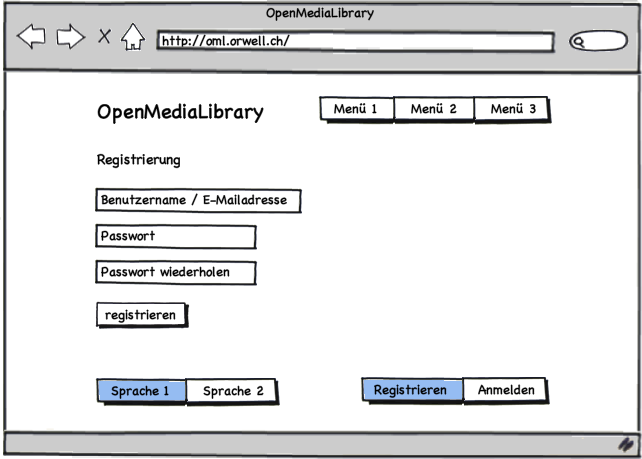
\includegraphics[width=1\textwidth,angle=0]{./wireframes/02_registrierung.png}
        \caption{Wireframe der Registrierung}
        \label{02_registrierung}
    \end{center}
\end{figure}

\begin{figure}[p]
    \begin{center}
        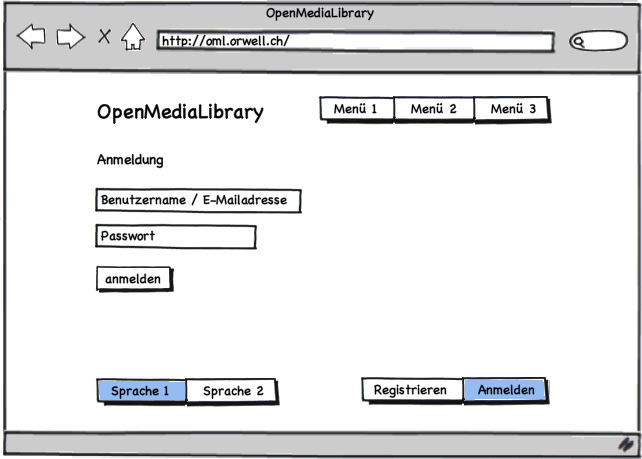
\includegraphics[width=1\textwidth,angle=0]{./wireframes/03_anmeldung.png}
        \caption{Wireframe der Anmeldung}
        \label{03_anmeldung}
    \end{center}
\end{figure}

\begin{figure}[p]
    \begin{center}
        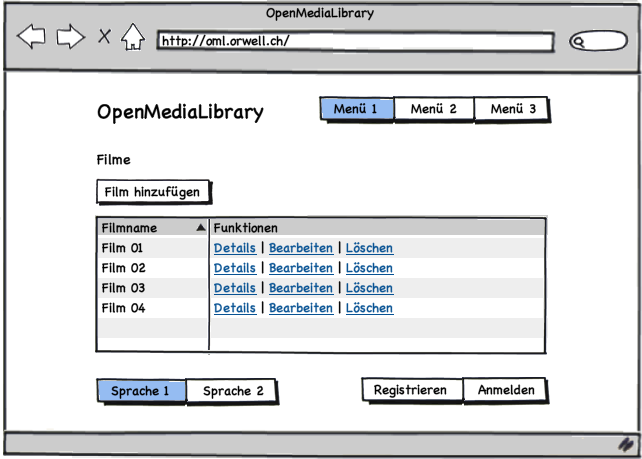
\includegraphics[width=1\textwidth,angle=0]{./wireframes/04_01_uebersicht.png}
        \caption{Wireframe der Filmübersicht}
        \label{04_01_uebersicht}
    \end{center}
\end{figure}

\begin{figure}[p]
    \begin{center}
        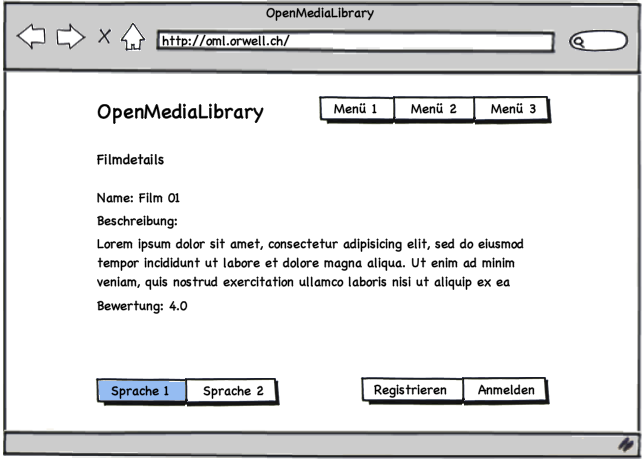
\includegraphics[width=1\textwidth,angle=0]{./wireframes/04_02_detail.png}
        \caption{Wireframe einer Filmdetailansicht für Gäste und nicht angemeldete Benutzer}
        \label{04_02_detail}
    \end{center}
\end{figure}

\begin{figure}[p]
    \begin{center}
        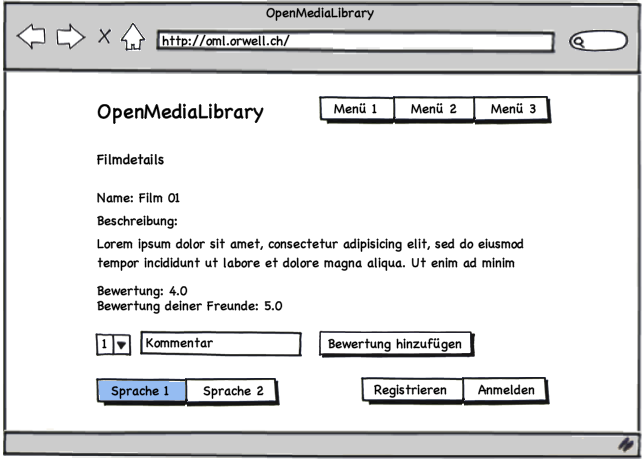
\includegraphics[width=1\textwidth,angle=0]{./wireframes/04_03_detail_angemeldet.png}
        \caption{Wireframe einer Filmdetailansicht für angemeldete Benutzer}
        \label{04_03_detail_angemeldet}
    \end{center}
\end{figure}

\begin{figure}[p]
    \begin{center}
        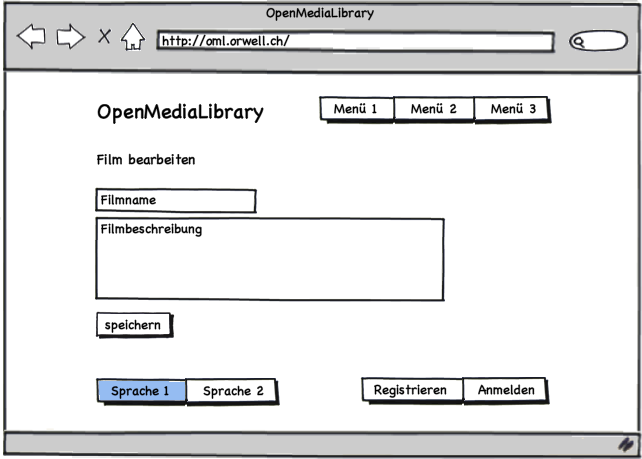
\includegraphics[width=1\textwidth,angle=0]{./wireframes/04_04_edit.png}
        \caption{Wireframe der Bearbeitungsmaske eines Filmes}
        \label{04_04_edit}
    \end{center}
\end{figure}

\clearpage

\section{Entity Relationship Model}
Aufgrund der definierten Funktionen und den Wireframes kann jetzt ein ER-Modell
erstellt werden. In der Grafik \ref{erm} ist das vollständige Modell des Prototypen
abgebildet.

Die Namen der Objekte sind in Englisch, da der Quellcode ausschliesslich in englischer 
Sprache geschrieben und kommentiert wird. Dies habe ich mit Absicht gewählt, 
damit es später für Drittentwickler keine unnötige Sprachbarriere gibt.

\begin{figure}[ht]
    \begin{center}
        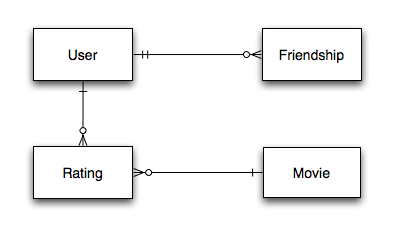
\includegraphics[width=0.6\textwidth,angle=0]{./erm/erm.png}
        \caption{ER-Modell des Prototypen}
        \label{erm}
    \end{center}
\end{figure}

In der Tabelle \ref{tab:erm} gehe ich auf die einzelnen Objekte des Modells ein
und erläutere ihre Funktion im Protoyp.

\begin{table}[ht]
\begin{center}
    \begin{tabular}{llp{10cm}l}
        \toprule Nr & Name & Funktion \\
        \midrule 1 & User & Bildet einen Benutzer im System ab. Ein Benutzer
                     kann keine bis mehrere Freunde (Friendship) haben. \\
        \midrule 2 & Friendship & Bildet eine Freundschaft zwischen genau zwei
                     Benutzern im System ab. Zu einer akzeptierten Freundschaft 
                     gehören immer genau zwei Benutzer. \\
        \midrule 3 & Rating & Bildet eine Bewertung eines Filmes, eines Benutzers
                     im System ab. Ein Benutzer kann mehrere Filme bewerten und
                     somit keine bis mehrere Bewertungen haben und eine 
                     existierende Bewertung gehört immer genau zu einem Benutzer 
                     und einem Film (Movie). \\
        \midrule 4 & Movie & Bildet einen Film im System ab. Ein Film kann keine
                     oder mehrere Bewertungen erhalten. \\
        \bottomrule
    \end{tabular}
    \caption{Erläuterungen zu den Objekten im ER-Modell}
    \label{tab:erm}
\end{center}
\end{table}

\clearpage

\section{Objektattribute}
Die Objekte im System haben genau definierte Attribute. Gewisse Attribute sind
statisch zum Objekt abgelegt, andere werden dynamisch berechnet. Da dies einen
Einfluss auf die Programmierung des Prototypen hat, werden diese explizit 
unterschieden.

In der Tabelle \ref{tab:attribute} liste ich alle Attribute
der einzelnen Objekte auf, beschreibe ihre Funktion und kennzeichne sie mit
einem `S' für statisch und einem `D' für dynamisch. Die Namen der Attribute sind 
ebenfalls ausschliesslich in englischer Sprache.

\begin{table}[ht]
\begin{center}
    \begin{tabular}{lllcp{9cm}l}
        \toprule Nr & Objekt & Attribut & Art & Funktion \\
        \midrule
            1 & User & Username & S & Beinhaltet den Benutzernamen des Benutzer. \\
            & & Password & S & Beinhaltet das Passwort des Benutzers. \\
            & & Ratings & D & Gibt alle Bewertungen des Benutzers zurück. \\
            & & Pending Friends & D & Gibt alle Freunde zurück, wo die Freundschaftsanfragen
                                      des Benutzers noch offen ist. \\
            & & Direct Friends & D & Gibt alle Freunde zurück, wo die Freundschaftsanfragen
                                     des Benutzers bereits akzeptier wurde. \\
            & & Inverse Friends & D & Gibt alle Freunde zurück, wo die Freundschaftsanfrage,
                                      die an den Benutzer gestellt worden sind, vom Benutzer
                                      akzeptiert wurden. \\
            & & Friends & D & Gibt alle Freunde, wo die Freundschaftsanfrage akzeptiert wurde,
                              egal ob die Freundschaftsanfrage direkt oder indirekt gestellt
                              wurde, zurück. \\
        \midrule
            2 & Friendship & User & S & Beinhaltet den Benutzer, der die Freundschaftsanfrage
                                        gestellt hat. \\
            & & Friend & S & Beinhaltet den Benutzer, an den die Freundschaftsanfrage gestellt
                                        wurde. \\
            & & Approved & S & Beinhaltet, ob die Freundschaftsanfrage akzeptiert wurde oder nicht. \\
        \midrule
            3 & Rating & User & S & Beinhaltet den Benutzer, der die Bewertung erfasst hat. \\
            & & Movie & S & Beinhaltet den Film, der bewertet wurde. \\
            & & Value & S & Beinhaltet die eigentliche Bewertung, also eine ganze Zahl zwischen 1 und 10. \\
            & & Comment & S & Beinhaltet optional einen Kommentar des Benutzers zur Bewertung. \\
        \midrule
            4 & Movie & Title & S & Beinhaltet den Namen des Filmes. \\
            & & Description & S & Beinhaltet die Beschreibung des Filmes. \\
            & & Ratings & D & Gibt alle Bewertungen des Filmes zurück. \\
            & & Users & D & Gibt alle Benutzer zurück, die den Film bewertet haben. \\
            & & Rating All & D & Gibt den Mittelwert aller Bewertungen aller Benutzer zurück. \\
            & & Rating Friends & D & Gibt den Mittelwert aller Bewertungen der Freunde des 
                                 angemeldeten Benutzers zurück. \\
        \bottomrule
    \end{tabular}
    \caption{Erläuterungen zu den statischen und dynamischen Attributen der Objekte}
    \label{tab:attribute}
\end{center}
\end{table}

    
    \chapter{Technologien \& Tools}
    \section{Auswahl}
Welche Technologien kommen für das Konzipierte überhaupt in Frage. Mit
was für Tools müsste man dazu arbeiten.

\section{Evaluation}
Bewertung der Technologien mit Gewichtung auch in Hinblick auf die Tools.

\section{Konklusion}
Für welche Technologien udn Projektunterstützende Tools man sich 
entschieden hat.
    
    \chapter{Prototyp}
    \section{Entwicklungsinfrastruktur}

\subsection{Entwicklungsumgebung}
MacOS X, Textmate, Terminal

\subsection{Versionierungssystem}
git develop, master

\subsection{Deployment}
Systeme: local, staging, production\\
Datenbanken: sqlite, mysql

\section{Umsetzung}

\section{Testen}

\subsection{Testfälle}

\subsection{Testresultate}
    
    \chapter{Konklusion}
    \section{Weiterentwicklung}

\section{Erfahrungsbericht}
    
    \appendix
    
    \chapter{Personalienblatt}
    \begin{tabbing}
	\hspace*{4cm}   \= \kill
	Name, Vorname:  \> {\bf Spross, Silvan} \\
	Adresse:        \> {\bf Meinrad Lienert-Strasse 27} \\
	PLZ, Wohnort:   \> {\bf 8003 Zürich} \\
	\\
	Geburtsdatum:   \> {\bf 07.11.1985} \\
	Heimatort:      \> {\bf Zürich ZH} \\
\end{tabbing}
    
    \chapter{Bestätigung}
    Hiermit bestätige ich, Silvan Spross, dass ich die vorliegende Semesterarbeit
``Webapplikation für eine öffentliche Medienbibliothek mit einer API'' im
Rahmen der geltenden Reglemente selbstständig ausgeführt habe.\\
\\
Zürich, den 29. Dezember 2010\\
\\\\
Silvan Spross
    
    \listoffigures

    \listoftables
    
    \bibliographystyle{ieeetr}
    \bibliography{referenzen}
    
\end{document}